\section{Результаты работы программы}

В верхней части окна показаны номер правила и его битовое представление.
По умолчанию открывается пустое поле размером $50\times50$. Если поле не
помещается в окне, его можно прокручивать. Главное окно показано на
рисунке~\ref{fig:application-window}.

\begin{figure}[H]
    \centering
    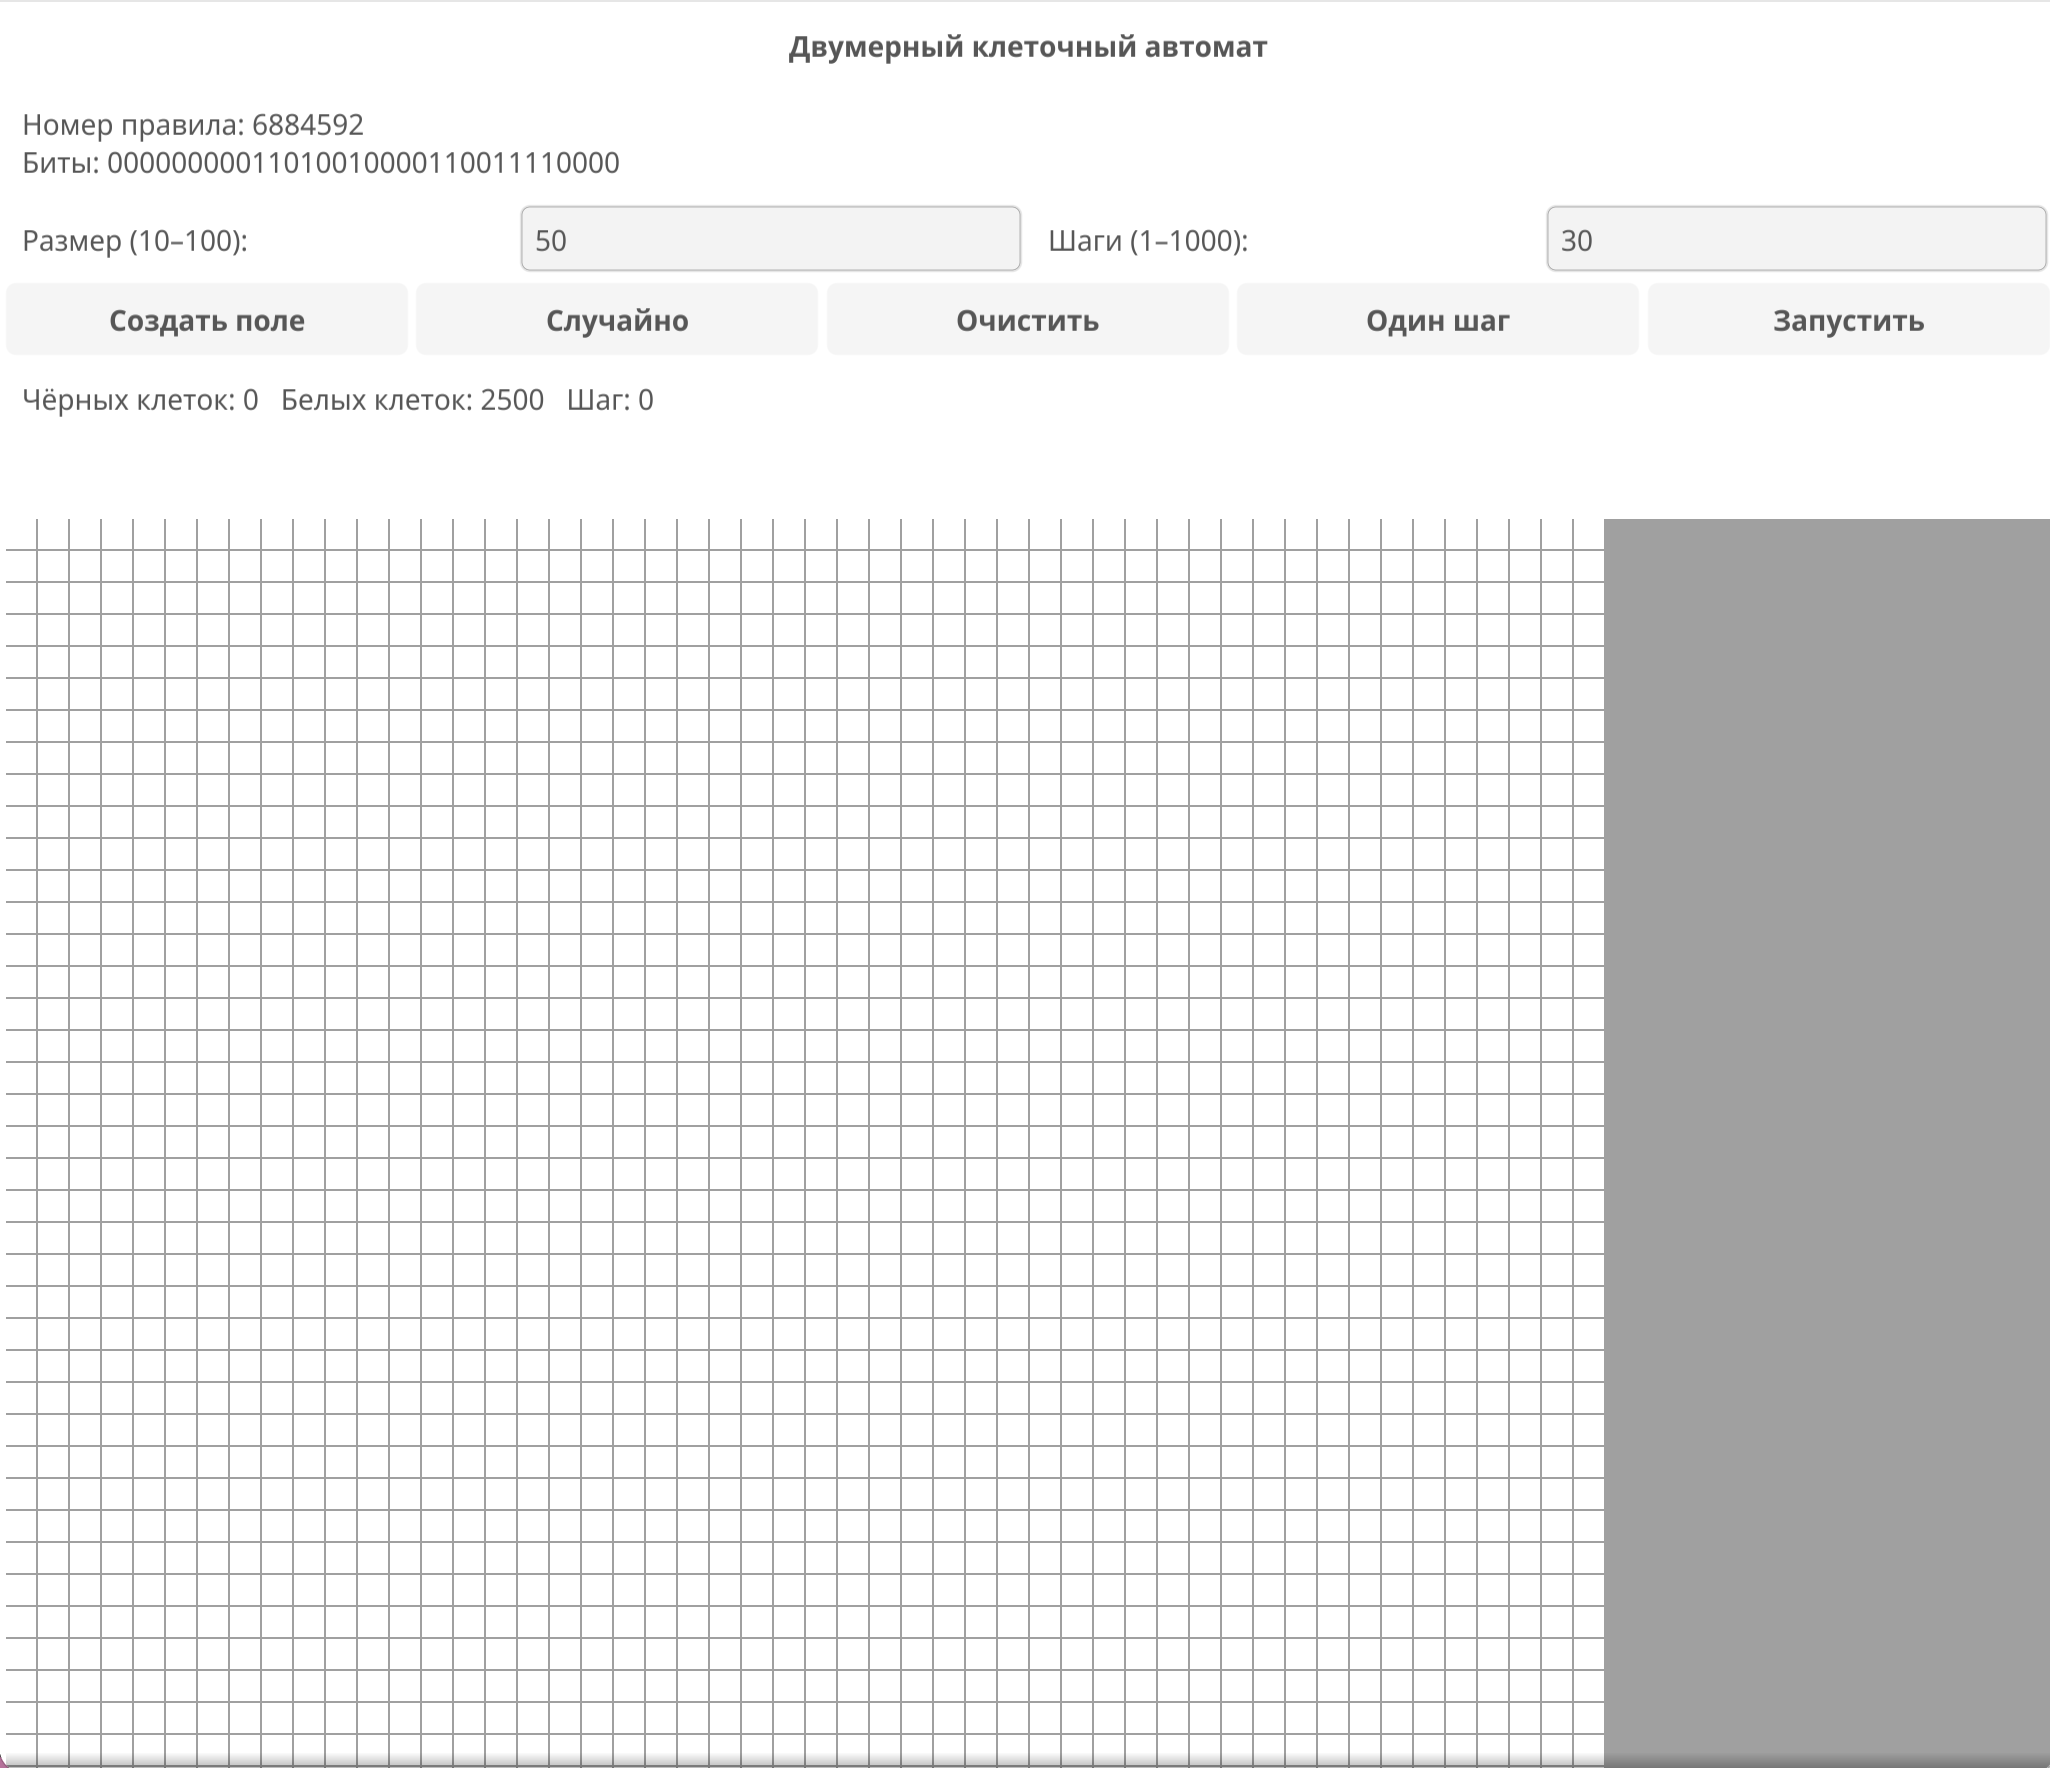
\includegraphics[width=0.9\linewidth]{myPhoto/results-empty-field.png}
    \caption{Пустое поле после запуска программы}
    \label{fig:application-window}
\end{figure}

Размер поля задаётся от 10 до 100 клеток по стороне (по умолчанию 50),
количество шагов - от 1 до 1000 (по умолчанию 30). Кнопка «Создать поле»
создаёт пустое поле выбранного размера.
Кнопки «Случайно» и «Очистить» задают случайное заполнение или делают все
клетки мёртвыми. Нажатие на клетку переключает её состояние. Пример случайного
заполнения поля приведён на рисунке~\ref{fig:application-initial-state}.

\begin{figure}[H]
    \centering
    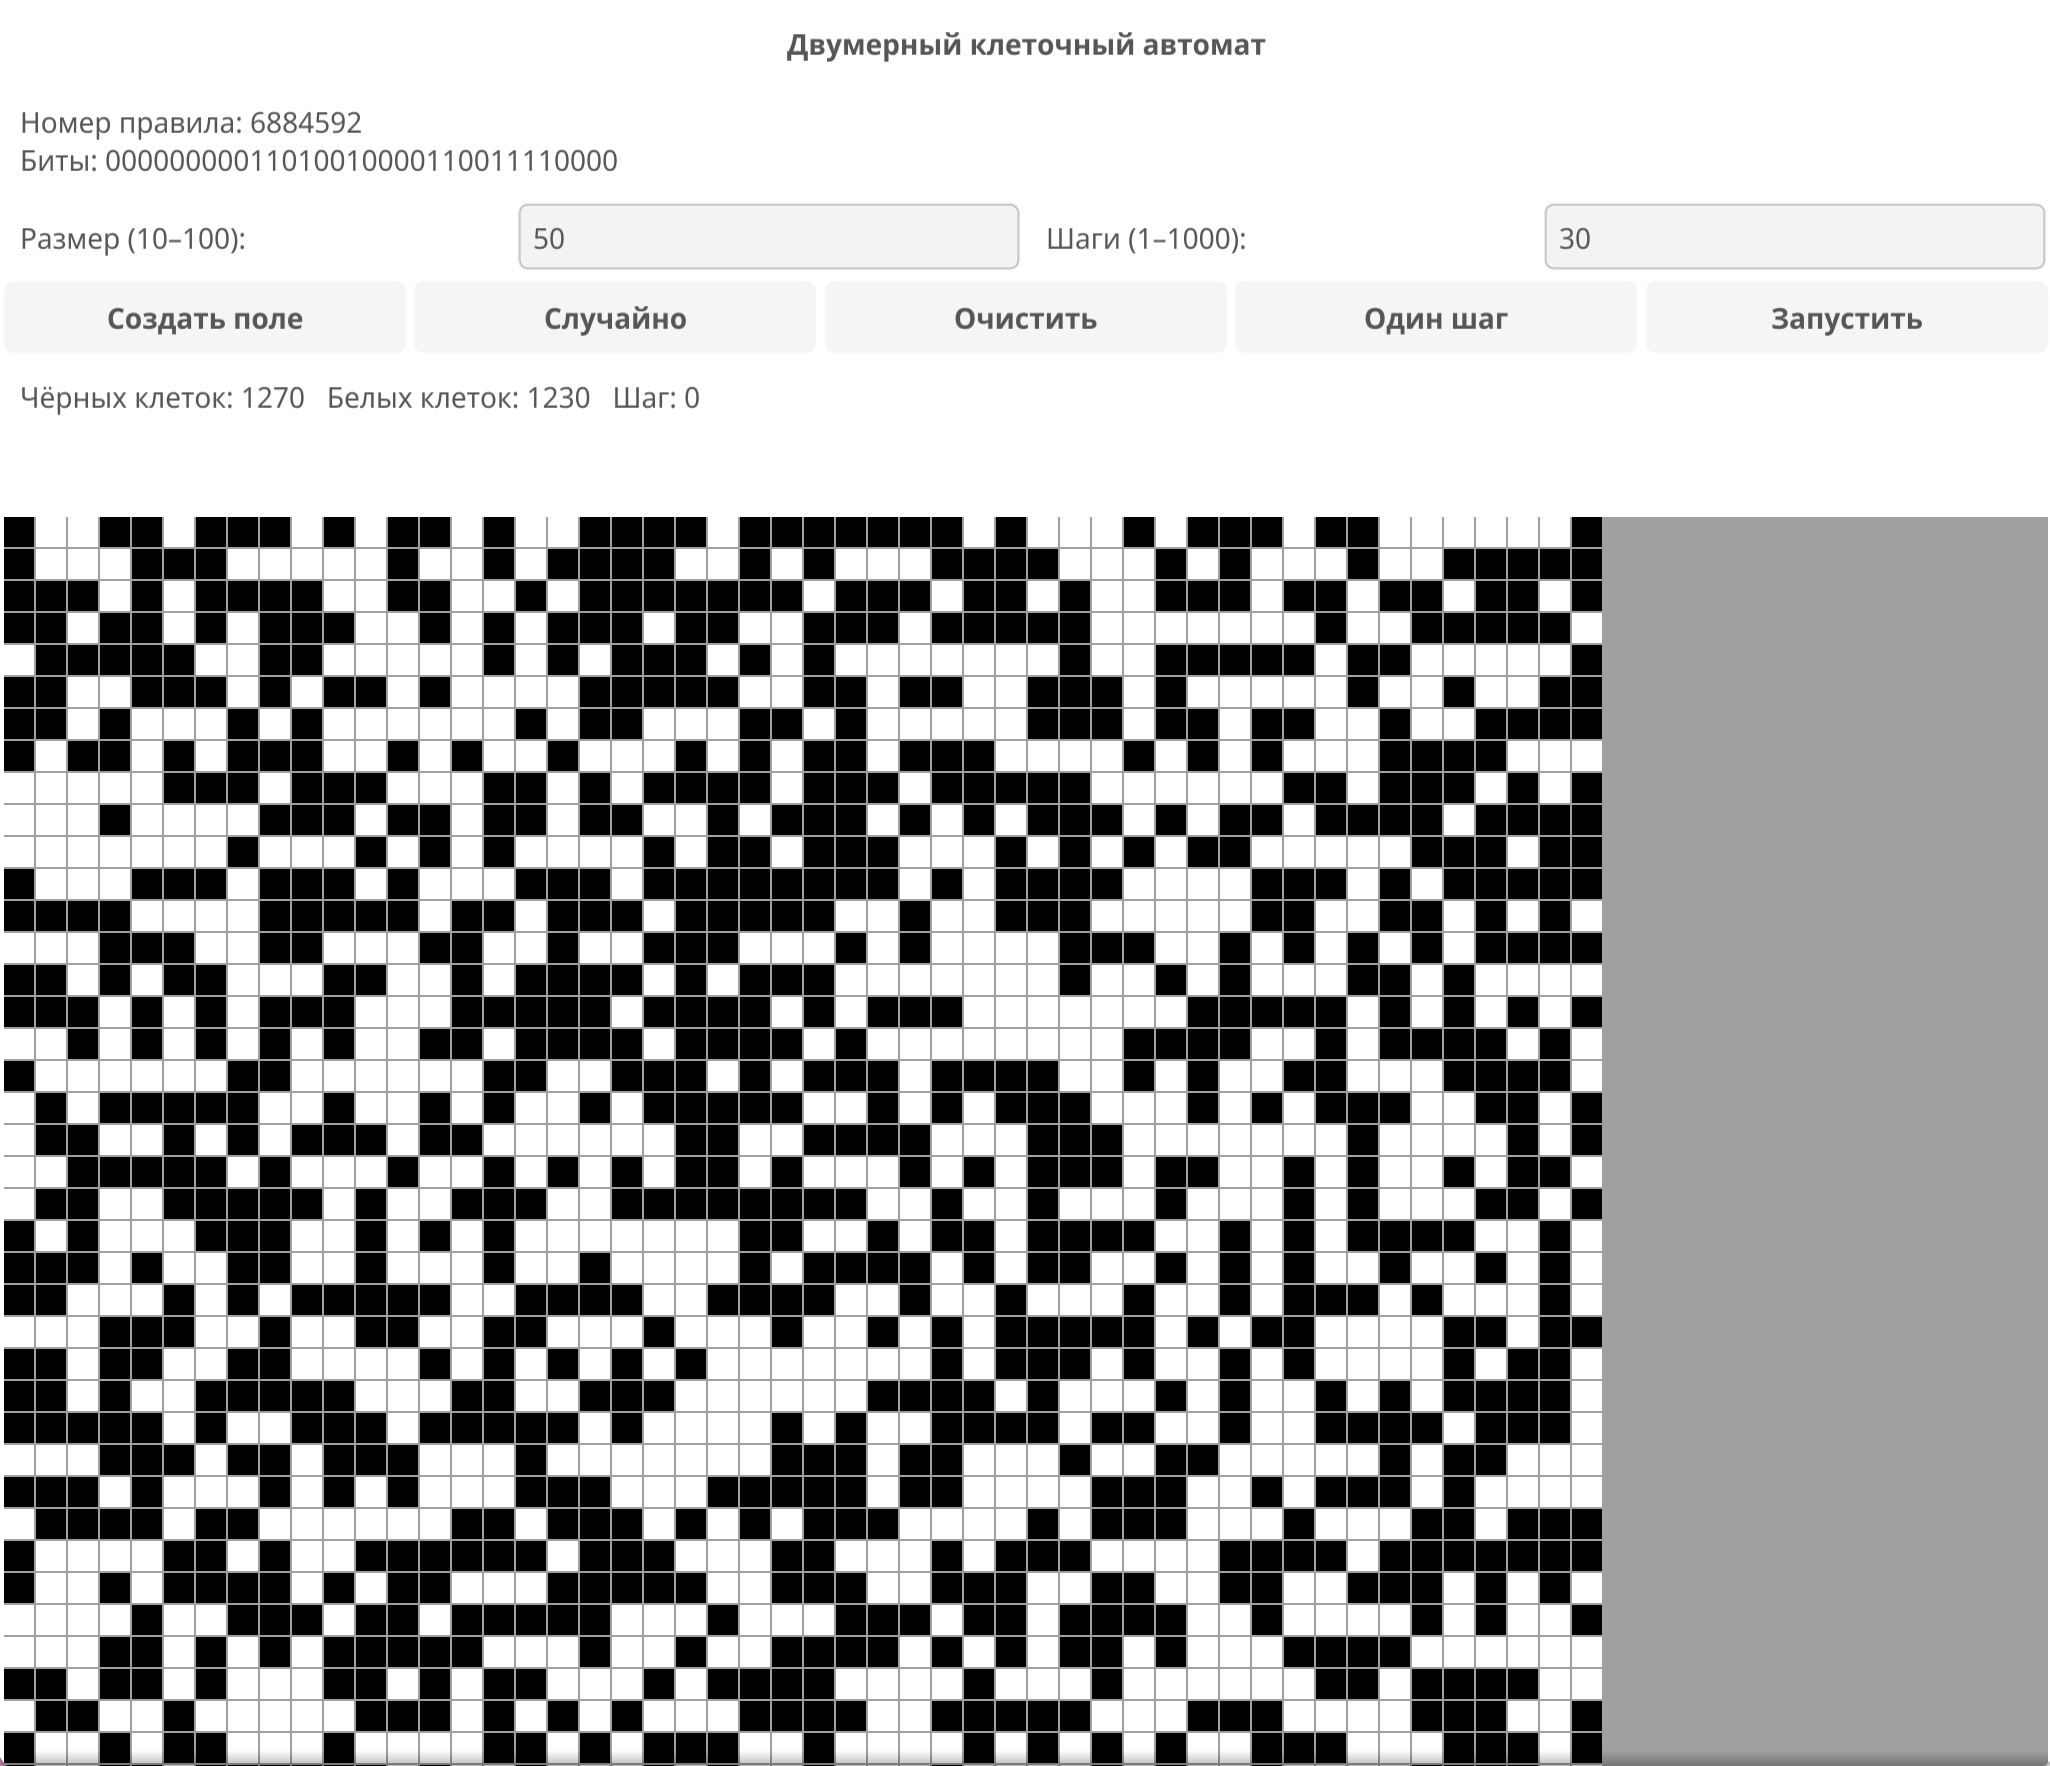
\includegraphics[width=0.9\linewidth]{myPhoto/results-random-field.png}
    \caption{Поле после случайного заполнения}
    \label{fig:application-initial-state}
\end{figure}

Кнопка «Один шаг» обновляет поле один раз. Кнопка «Запустить» выполняет
заданное число шагов. Под кнопками отображаются количества чёрных и белых
клеток и номер текущего шага. Результат выполнения 30 шагов показан на
рисунке~\ref{fig:application-result}.

\begin{figure}[H]
    \centering
    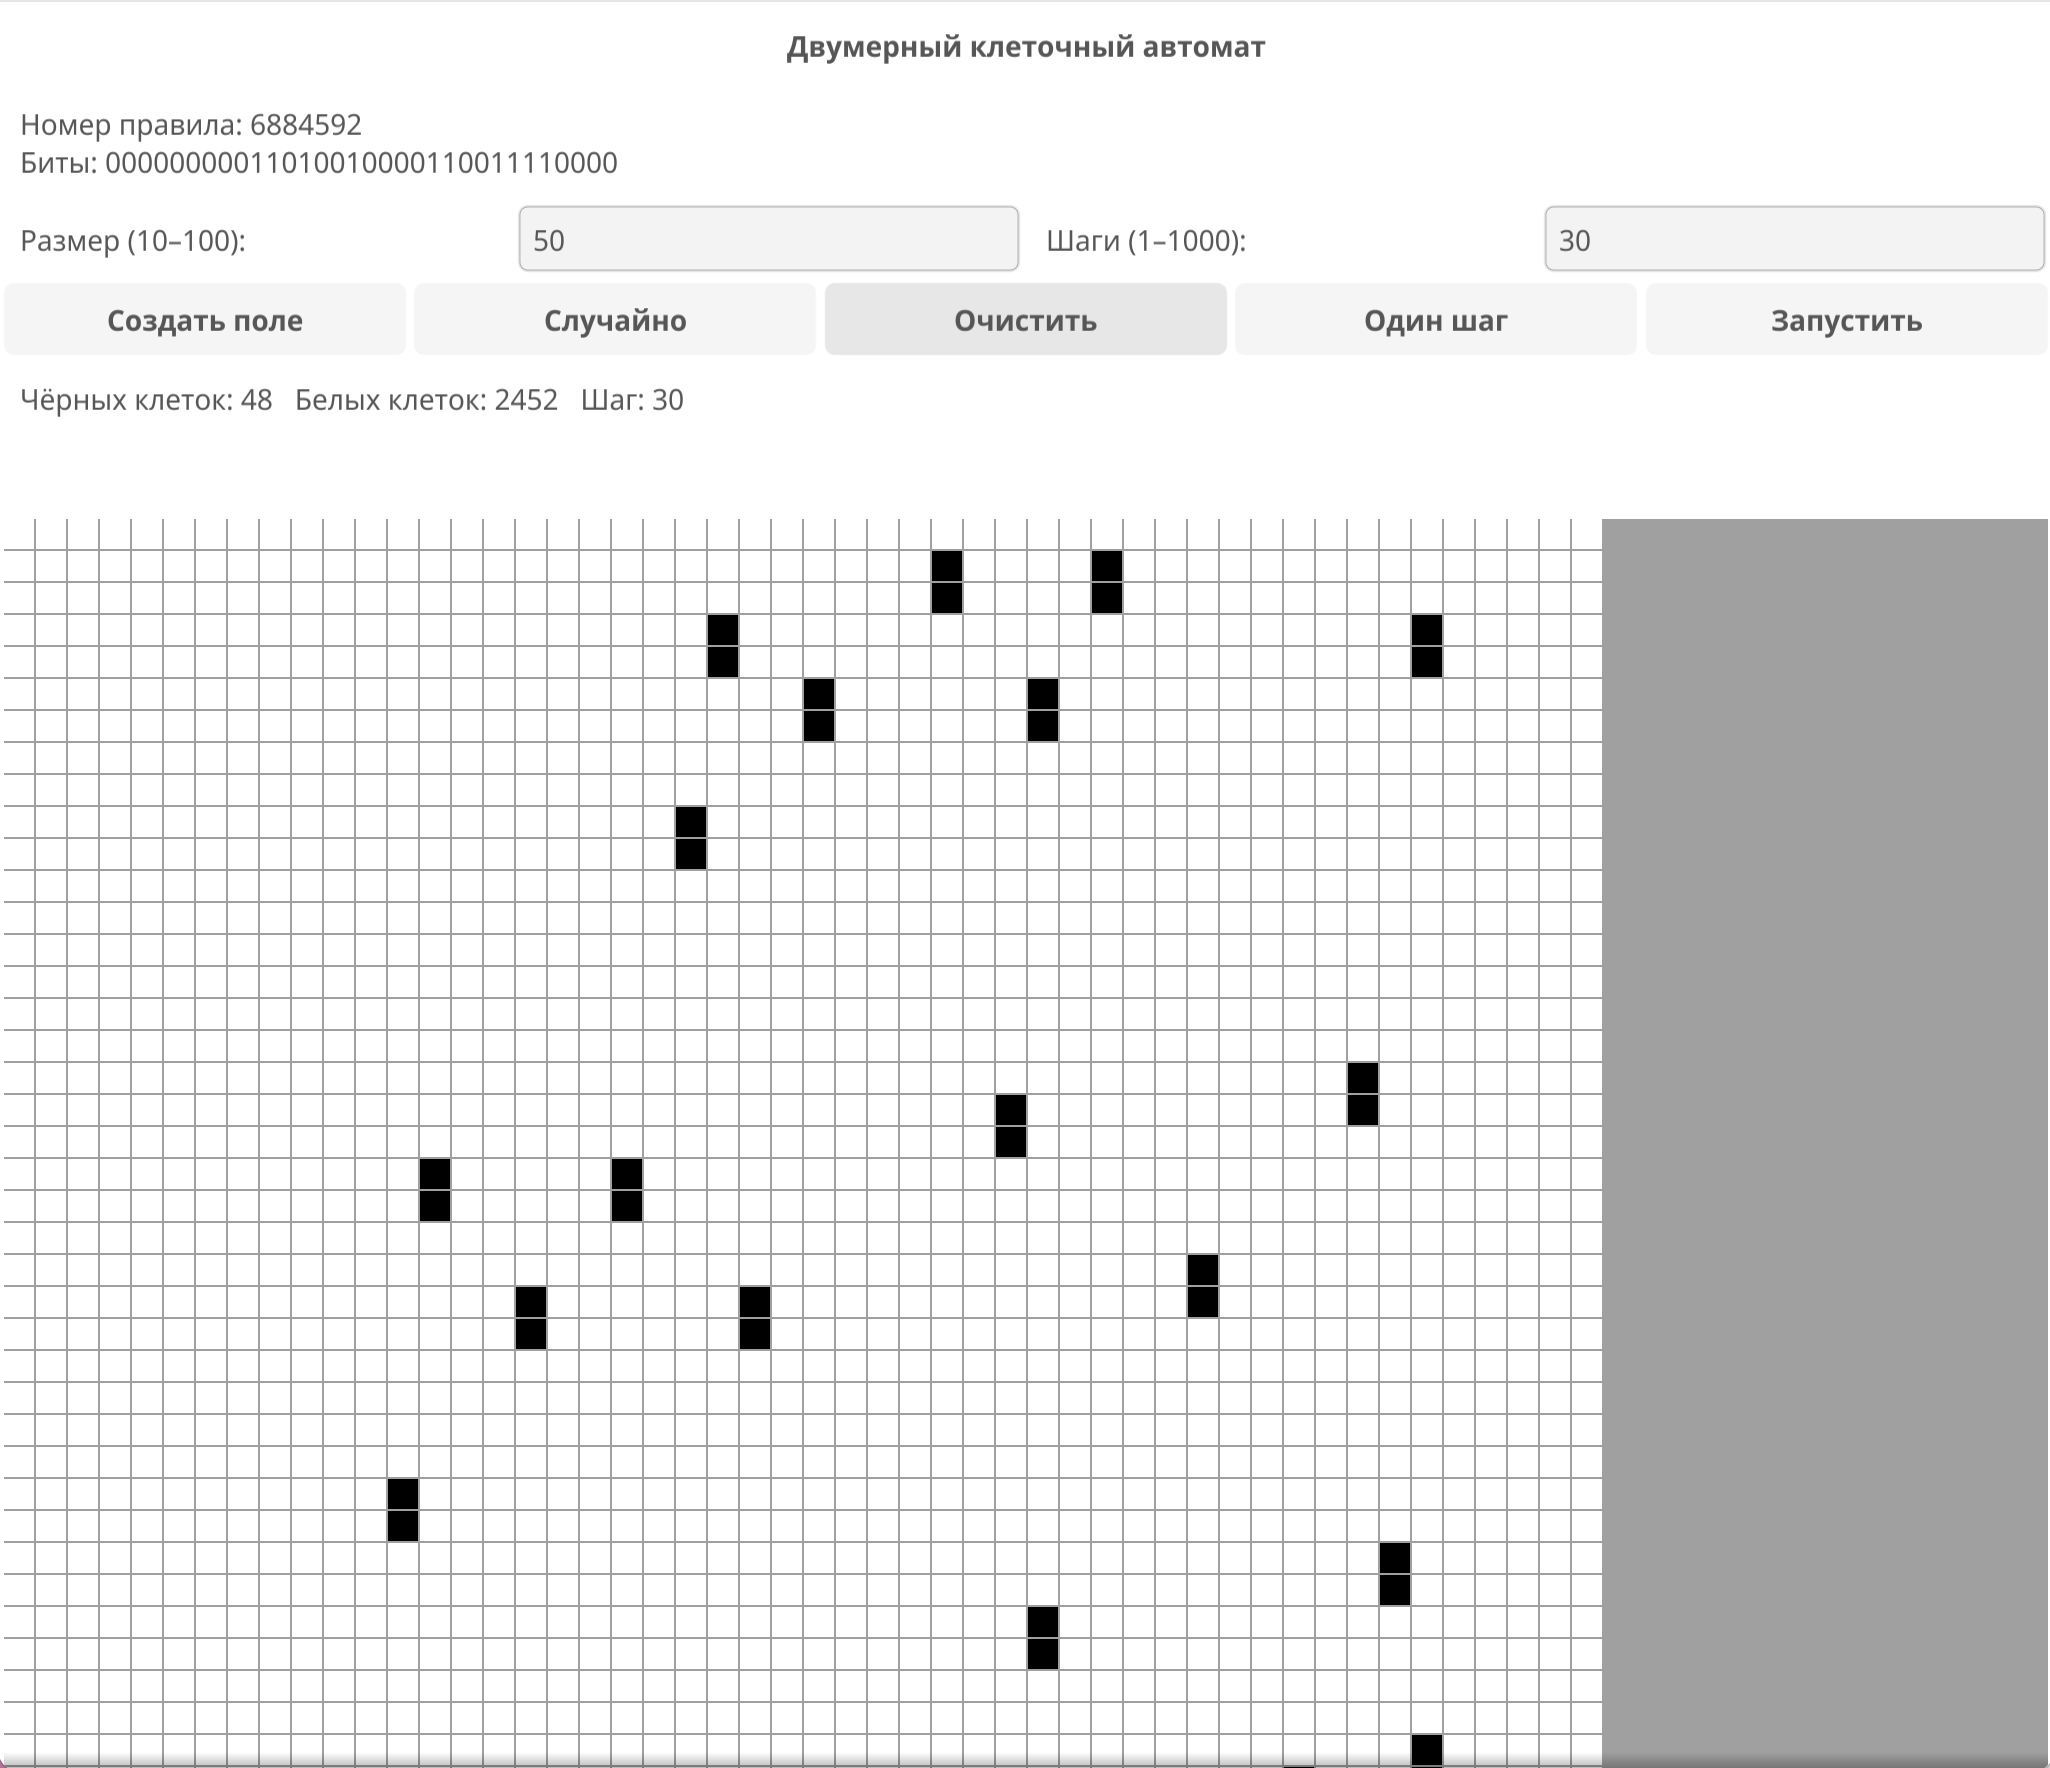
\includegraphics[width=0.9\linewidth]{myPhoto/results-after-steps.png}
    \caption{Поле после выполнения 30 шагов автомата}
    \label{fig:application-result}
\end{figure}
